% !TeX spellcheck = en_US
% !TeX program = pdflatex

\documentclass[12pt,sans]{article}
\usepackage{cmap}
\usepackage[T2A]{fontenc}
\usepackage[utf8]{inputenc}
\usepackage[english]{babel}

%\usepackage{paratype}
\usepackage{PTSans}
\renewcommand{\rmdefault}{\sfdefault}
\usepackage{euler}
\usepackage{ifthen}
\usepackage[most]{tcolorbox}

\usepackage{amsthm,amsmath,amssymb}
\usepackage{xspace}
\usepackage{fullpage}
\usepackage{comment}

%% CALCULATOR
\usepackage{calc}
%% STYLE
\usepackage[dotinlabels]{titletoc}
\usepackage[small]{titlesec}
%% TITLESEC BUG WORKAROUND %%
\usepackage{etoolbox}
\makeatletter
\patchcmd{\ttlh@hang}{\parindent\z@}{\parindent\z@\leavevmode}{}{}
\patchcmd{\ttlh@hang}{\noindent}{}{}{}
\makeatother
%% END %%
\titlelabel{\thetitle.\quad}
%% Puts ``.'' instead of ``:'' in captions
\usepackage{ccaption}
\captiondelim{. }

\usepackage{indentfirst}

\usepackage[mathlines]{lineno}
\linenumbers
%% OTHER

\usepackage[bookmarks=false, colorlinks, unicode, pdfstartview=FitH, pdftex
]{hyperref}
\hypersetup{
 plainpages=true,
 linkcolor=blue,
 citecolor=red,
 menucolor=blue,
 pdfnewwindow=true
}

\usepackage{tikz}
\usetikzlibrary{positioning,calc}

\newcommand{\bits}{\{0,1\}}
\newcommand{\bitstr}{\bits^*}
\newcommand{\sshalf}{{\textstyle\frac12}}
\newcommand{\seqn}[2]{{#1}_1,{#1}_2,\dotsc,{#1}_{#2}}
\newcommand{\seqin}[3]{{#1}_{{#2}_1},{#1}_{{#2}_2},\dotsc,{#1}_{{#2}_{#3}}}
\newcommand{\IC}{\mathrm{IC}}
\newcommand{\poly}{\mathrm{poly}}
\newcommand{\Nat}{\mathbb{N}}

\DeclareMathOperator{\dom}{dom}
\DeclareMathOperator{\rank}{rank}
\DeclareMathOperator{\rng}{rng}
\DeclareMathOperator*{\E}{\mathbb{E}}

\theoremstyle{definition}
\newtheorem{definition}{Definition}[section]

\theoremstyle{plain}
\newtheorem{theorem}{Theorem}[section]
\newtheorem{lemma}{Lemma}[section]
\newtheorem{statement}{Statement}[section]
\newtheorem{corollary}{Corollary}[section]

\theoremstyle{remark}
\newtheorem{example}{Example}[section]
\newtheorem{exercise}{Exercise}[section]
\newtheorem{remark}{Remark}[section]
\newtheorem{problem}{Problem}[section]

\newboolean{forstudents}
\setboolean{forstudents}{false}

\definecolor{block-gray}{gray}{.9}
\newtcolorbox{solutionblock}{colback=block-gray,grow to right by=-10mm,grow to left by=-10mm,
    boxrule=0pt,boxsep=0pt,breakable}

\ifthenelse{\boolean{forstudents}}{\excludecomment{solution}}{%
\newenvironment{solution}{%
    \begin{solutionblock}\emph{Solution.}
    }{%
    \end{solutionblock}
}}


\newenvironment{tasks}{\paragraph{Problems.}\begin{enumerate}}{\end{enumerate}}

%opening
\title{Notes on Information Theory}
\author{Alexander V. Smal}
\begin{document}

\maketitle

\begin{abstract}
    This course is dedicated to studying approaches to defining the concept of ``quantity of information''. The sequence of material presentation is based on Kolmogorov's classic article ``Three Approaches to the Definition of the Concept of Quantity of Information'' (1965).

    The course will cover three approaches to defining ``quantity of information'':
    \begin{itemize}
        \item Combinatorial (information by Hartley)
        \item Probabilistic (Shannon entropy)
        \item Algorithmic (Kolmogorov complexity)
    \end{itemize}

    In addition, we will discuss various applications of information theory in different fields of computer science: in cryptography, communication complexity, coding theory, finite automata theory, computational complexity theory, and others.
\end{abstract}

\newpage\tableofcontents\newpage

\section{Combinatorial Approach}
\subsection{Hartley's definition}
Let a finite set \(A\) be given—\emph{the set of outcomes}.
\begin{definition}[1928]
    We define \emph{the amount of information in \(A\)} as \(\chi(A) = \log_{10}|A|\).
\end{definition}

According to this definition a set of size 10 has 1 unit of information.
Note that the base of algorithm can be different.

If it becomes known for some \(x\in A\) that \(x\in B\), then to identify \(x\) we now need \(\chi(A\cap B) = \log |A\cap B|\) bits, i.e., we have been informed \(\chi(A) - \chi(A\cap B)\) bits of information.

\begin{example}
    Suppose we want to discover some unknown ordering of the set $\{\seqn{a}{5}\}$. We have learned that \(a_1>a_2\) or \(a_3>a_4\). How many bits of information have we gained? The set \(A\) consists of \(5!\) permutations, while the set \(B\) consists of the permutations that satisfy the new condition. It is easy to verify that \(|B| = 90\). Thus, we have learned \(\log 120 - \log 90 = \log(4/3)\) bits.
\end{example}

Let \(A\subset\bitstr\times\bitstr\). Denote by \(\pi_1(A)\) and \(\pi_2(A)\) the projections of the set \(A\) onto the first and second coordinates, respectively, and let \(\chi_1(A) = \log|\pi_1(A)|\) and \(\chi_2(A) = \log|\pi_2(A)|\) be the quantity of information in them according to Hartley.

\begin{theorem}
    \(\chi(A) \le \chi_1(A) + \chi_2(A)\).
\end{theorem}

\begin{definition}
    The quantity of information in the second coordinate of \(A\subset\bitstr\times\bitstr\) given the first is
    \[\chi_{2|1} = \log\max_{a\in\pi_1(A)}\bigl|\{x \mid (a, x)\in A\}\bigr|.\]
\end{definition}

\begin{theorem}
    \(\chi(A) \le \chi_1(A) + \chi_{2|1}(A)\).
\end{theorem}

\begin{theorem}\label{thm:volume}
    For \(A\subset\bitstr\times\bitstr\times\bitstr\)
    \[2\cdot\chi(A) \le \chi_{12}(A) + \chi_{13}(A) + \chi_{23}(A).\]
\end{theorem}
\begin{corollary}
    The square of the volume of a three-dimensional body does not exceed the product of the areas of its projections onto the coordinate planes.
\end{corollary}

\begin{statement}
    If \(f: X\to Y\)
    \begin{enumerate}
        \item is a surjection, then \(\chi(Y)\le \chi(X)\),
        \item is an injection, then \(\chi(X)\le \chi(Y)\).
    \end{enumerate}
\end{statement}

\subsection{Application: The Game of 10 Questions}
How many yes/no questions need to be asked to determine a secret number from 1 to \(N\), if (a) questions can be asked adaptively; (b) questions must be written down in advance.

The estimate \(\lceil\log N\rceil\) is achieved in both cases if questions about the bits of the binary representation of the secret number are asked.

Let's prove the lower bound. Let \(A=[N]\). The set \(Q = \{(\seqn{q}{k})\}\) is the set of protocols (answers to the questions). We can consider \(A\) and \(Q\) as projections of some outcome set of the game \(S\) onto different coordinates. Then the following inequalities hold:
\begin{itemize}
    \item \( \chi_Q(S) = \chi(Q) \le \chi_1(Q) + \chi_2(Q) + \dotsb + \chi_k(Q) \le k, \)
    \item \( \chi_A(S) = \chi(A) \le \chi(S) \le \chi_Q(S) + \chi_{A|Q}(S) \le k + 0 = k. \)
\end{itemize}
Thus, we obtain \(\log N = \chi(A) \le k\).

\subsection{Cost of Information}
Let a secret integer be chosen from 1 to \(n\) (where \(n \ge 2\)).
Any yes/no questions can be asked. For a positive answer, we will pay 1 ruble, and for a negative answer—two rubles. How much is necessary and sufficient to guess the number?

\paragraph{Upper Bound.} We will ask questions in such a way that negative answers provide twice as much information as positive ones. Then for each bit of information, we will pay a constant amount of rubles \(c\). Let all questions be of the form “is \(x \in T\)?”. We require that
\[2\cdot(\log |X| - \log|X \cap T|) = \log |X| - \log|X\cap\overline T|.\]
Let \(|X \cap T| = \alpha|X|\), then \(|X\cap\overline T| = (1 - \alpha)|X|\),
thus we obtain the equation
\[2\log (1/\alpha) = \log (1/(1-\alpha)),\]
equivalent to the quadratic equation
\[\alpha^2 = 1 - \alpha.\] Among the two roots, we are interested in the one that is less than 1, i.e., \(\alpha=(\sqrt 5 - 1) / 2\). Therefore, for any answer, we will pay \(c = 1/(-\log \alpha)\approx 1.44\) rubles per bit, and in total—\(c\log n\) rubles.

In this estimate, we have completely ignored rounding questions. Indeed, we can never divide a set of \(n\) elements into two in the ratio \(\alpha:(1-\alpha)\), since \(\alpha\) is irrational. Therefore, some rounding error will accumulate with each question. Instead of questions about membership in a certain subset \(T\) of the set \(X\), let's ask about membership in an interval with real coordinates. We start with the interval \(S = [1,n]\) and will reduce it by a factor of \(1/\alpha\) each time, i.e., we will first ask whether \(x\) belongs to the interval \(S' = [1, 1 + \alpha(n-1)]\). The length of the interval \(S'\) is \(1/\alpha\) times less than the length of the interval \(S\). We will continue in this manner until the length of the interval becomes less than 1—in this case, \(x\) is uniquely defined. After each question, the length of the interval decreases at most by a factor of \(1/(1 - \alpha) = 1/\alpha^2\), so the length of the last interval is at least \(\alpha^2\). Thus, the length of the interval will not reduce by more than \((n-1)/\alpha^2\) times. Since we chose the intervals each time so that we pay \(c\) rubles for a decrease of \(\log |S|\) by 1, we will pay in total no more than
\[
c\log((n-1)/\alpha^2) = c\log(n-1) - 2c\log \alpha = c\log(n-1) + 2.
\]
In any outcome, we will pay a whole number of rubles, so this estimate can be refined to \(\lfloor c\log(n-1)\rfloor + 2\).

\paragraph{Lower Bound.} We will apply the adversary argument. Let the adversary
choose the answer YES/NO depending on which of the two values \(1/(\log |X| - \log|X \cap T|)\) and \(2/(\log |X| -
\log|X \cap \overline T|)\) is greater. For any \(X,\ T\), one of these values is at least \(c = 1/(-\log\alpha)\). Thus,
we force the algorithm to pay at least \(c\) rubles per bit, meaning that any algorithm in the worst case will pay
\(\lceil c\log n\rceil\) rubles.

\subsection{Application: Sorting Stones by Weight}
\subsubsection{Upper and Lower Bounds for Arbitrary \(N\)}
How many comparisons are needed to sort \(N\) stones by weight?

\paragraph{Lower Bound.} It will require \(\lceil\chi(S_N)\rceil = \lceil\log n!\rceil\) comparisons.

\paragraph{Upper Bound.} We will sort using insertion sort with binary search for the insertion point. The number of comparisons is:
\[
\lceil\log 2\rceil + \lceil\log 3\rceil + \dotsb + \lceil\log n\rceil \le \log n! + n - 1 = n\log n + O(n).
\]

\subsubsection{Exact Estimates for Small \(N\)}
\begin{exercise}
    How many weighings are needed to sort \(N\) stones by weight?
    Find the exact answer to this question for \(N = 2, 3, 4, 5\). Hint: use a greedy strategy where each weighing provides maximum information.
\end{exercise}

\subsection{Application: Finding the Fake Coin}
The following problems are proposed.
\begin{itemize}
    \item There are 20 visually identical coins, one of which is fake and lighter than the others.
    How can you find the fake coin using a balance scale? What is the minimum number of weighings needed?

    \textit{Solution.} Each weighing provides at most \(\log 3\) bits of information, so the number of weighings is at least $\lceil\log 20 / \log 3\rceil = \lceil\log_3 20\rceil = 3$.

    \item There are 13 visually identical coins, one of which is fake (with unknown relative weight).
    Can you find the fake coin and determine its relative weight in three weighings?

    \begin{solution}
        We need to consider two options for the first step:
    \begin{itemize}
        \item If we weigh 4 coins, then if they are equal, we cannot find the fake coin among 5 in two weighings (10 outcomes remain),
        \item If we weigh 5 coins, then if they are unequal, 10 possible outcomes remain.
    \end{itemize}
    \end{solution}

    \item There are 15 visually identical coins, one of which is fake. Can you find the fake coin in three weighings
    if you do not need to determine its relative weight?

    \textit{Solution.} Let's consider how many different outcomes there can be. The only case in which we can identify the fake coin without knowing its relative weight is if it has never been on the scale. This means that in all three weighings, the scale will be balanced. Therefore, there can be only one such coin, and in other cases, we will know the relative weight. In such a case, the number of different outcomes is \(2\cdot 14 + 1 = 29\), which exceeds \(3^3\)~— the number of results of three weighings.

    \item There are 14 visually identical coins, one of which is fake. Can you find the fake coin in three weighings
    if you do not need to determine its relative weight?

    \textit{Instead of a solution.} Similar reasoning does not allow proving impossibility, since \(2\cdot 13 + 1 = 3^3\).
    Nevertheless, it is impossible to solve this problem in three weighings. To prove this, we need more than
    the definition of information by Hartley.

\end{itemize}

\begin{exercise}
    Find one fake coin among 12 in three weighings, if its relative weight is unknown. Hint: use a ``greedy'' strategy, where each weighing provides maximum information.
\end{exercise}

\begin{exercise}
    Let \(L_n\) be the set of paths of length \(n\) in a graph.
    \begin{center}
        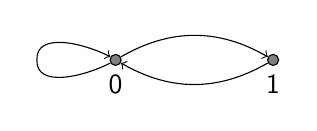
\begin{tikzpicture}
            \tikzstyle{vert}=[circle, draw, fill=black!50,
            inner sep=0pt, minimum width=4pt]
            \node[vert, label=below:0] (a) at (1,0) {};
            \node[vert, label=below:1] (b) at (3,0) {};
            \node (c) at (0,0) {};
            \path
            (a) edge [->,bend left] (b)
            (b) edge [->,bend left] (a)
            (a) edge [bend left, in=90] (0,0)
            (0,0) edge [->,bend left,out=90] (a);
        \end{tikzpicture}
    \end{center}
    What is the limit \(\lim_{n\to\infty} \frac{\chi(L_n)}{n}\)?
\end{exercise}

\begin{exercise}
    Let a number be chosen from 1 to \(N\). You can ask any yes/no questions. How many questions will be needed if one answer can be incorrect, and the questions (a) can be asked adaptively; (b) need to be written in advance?
\end{exercise}

\subsection{Logic of Knowledge}
In this section, we will refer to a set of outcomes \(A\) as a set of \emph{worlds}.
Let \(f\) be some function from \(A\) to a set \(I\) (we will perceive this as information about the world).
We are not concerned with the specific values that \(f\) takes; rather, we will focus on the equivalence classes into which \(f\) divides \(A\):
each equivalence class will consist of worlds in \(A\) with the same value of \(f\).

\begin{example}
    Let \(A = \{1,2,3,4,5\}\), and \(f(x) = x \bmod 3\). Then \(f\) divides \(A\) into three equivalence classes
    \(\{1,4\}\), \(\{2,5\}\), and \(\{3\}\).
\end{example}

Let \(B \subset A\) be some \emph{statement} about the worlds. \(B\) is \emph{true} in world \(x\) if \(x \in B\).
Otherwise, \(B\) is \emph{false} in \(x\). In world \(x\), we \emph{know that \(B\) is true} if \(y \in B\) for all
\(y \sim x\).

\begin{example}
    Let \(A = \{1,2,3,4,5\}\), and \(f(x) = x \bmod 3\). Then in worlds \(1\), \(4\), and \(3\) we know that the world is less than \(5\).
    In worlds \(2\) and \(5\) we do not know.
\end{example}
\begin{remark}
    By ``not knowing,'' we will mean ``it is not true that we know.''
\end{remark}

Common logical connectives can be applied to statements about worlds: ``AND'' (intersection), ``OR'' (union),
``NOT'' (complement).

\begin{statement}
    If in world \(x\) we know \(B\), then in world \(x\) we know that we know \(B\).
    Similarly, if in world \(x\) we do not know \(B\), then in world \(x\) we know that we do not know \(B\).
\end{statement}

Now suppose we have \(k\) people with their own knowledge about the world.
They define \(k\) equivalence relations \(\sim_1, \sim_2, \dotsc, \sim_k\) and,
accordingly, \(k\) partitions into equivalence classes.

\begin{example}
    Let the set of worlds \(A = \{1,2,3,4,5\}\) and there are two people, Alice and Bob.
    Alice knows the values \(f_A(x) = x \bmod 3\), while Bob knows \(f_B(x) = x \bmod 2\).
    Then Alice's equivalence classes are: \(\{1,4\}\), \(\{2,5\}\), and \(\{3\}\),
    while Bob's equivalence classes are: \(\{1,3,5\}\) and \(\{2,4\}\).
    In world 1, Alice knows that the world is less than 5, while Bob does not know. In world 4, both know this.
    In world 1, Alice does not know that Bob does not know that the world is less than 5 (indeed, in world 4,
    which is equivalent to 1 from Alice's perspective, Bob knows this).
\end{example}

\begin{exercise}
    Suppose there is a card known to have a non-negative integer \(n\) written on one side and the integer \(n+1\) on the other side.
    Alice and Bob are sitting opposite each other, looking at this card from different sides, and the following conversation occurs between them.
    \begin{itemize}
        \item[A:] I do not know the number on Bob's side.
        \item[B:] I do not know the number on Alice's side.
    \end{itemize}
    This is repeated 10 times, after which Alice says that she knows the number on Bob's side. What numbers could have been written on the card?
\end{exercise}

\begin{exercise}
    In a shop, there are three red hats and two white hats. Three gentlemen take turns buying a random hat and putting it on without looking
    (i.e., the gentleman does not know the color of the hat he bought). After this, the gentlemen look at each other and the following conversation occurs.
    \begin{itemize}
        \item[1:] I do not know the color of my hat.
        \item[2:] I do not know the color of my hat.
        \item[3:] Now I know the color of my hat.
    \end{itemize}
    What color is the hat on the third gentleman?
\end{exercise}

\begin{exercise}
    The king has 9 bottles of wine. One of the bottles contains poisoned wine.
    The king has two maids. Each day, any maid can mix a cocktail from different bottles in her glass and drink it, but each maid only gets one attempt per day, at a fixed time, exactly at noon (so if both maids try, one cannot take the result of the other into account on the same day). Any amount of poisoned wine in the glass will quickly kill.

    How can one discover which bottle is poisoned in two days?
\end{exercise}

\section{Probabilistic Approach}
\subsection{Shannon Entropy}

Shannon entropy defines the amount of information \(H(\alpha)\) in the probability distribution for a random variable \(\alpha\). Let \(\alpha\) take values from the set \(\{\seqn{a}{k}\}\) with probabilities \(\{\seqn{p}{k}\}\), where \(p_i \ge 0\) and \(\sum_i p_i = 1\).

We would like this definition to be consistent with Hartley's definition, i.e., the following ``boundary conditions'' hold:
\begin{itemize}
    \item if \(p_1 = \dotsb = p_k\), then \(H(\alpha) = \log k\),
    \item if \(p_1 = 1\), \(p_2 = \dotsb = p_k = 0\), then \(H(\alpha) = 0\).
\end{itemize}
We will seek \(H(\alpha)\) in the form of the expected value of the information we obtain from each outcome.
\[
H(\alpha) = \sum_i p_i \cdot \text{(information in $a_i$)}.
\]
How do we estimate how much information is in the outcome $a_i$? Let $U$ be the entire space of elementary outcomes, all of which are equally probable. Then, the event \(\alpha = a_i\) corresponds to a set of elementary outcomes with measure \(p_i\). Accordingly, if the event \(\alpha = a_i\) occurs, the size of the set corresponding to this event decreases from \(|U|\) to \(p_i |U|\), i.e., the event \(\alpha = a_i\) tells us \(\log |U| - \log (p_i |U|) = \log \frac{1}{p_i}\) bits of information.

Now let us assume the elementary outcomes are not equally probable. In this case, the event \(\alpha = a_i\) provides us with information that reduces the \emph{measure} of the set of possible outcomes by a factor of \(1/p_i\), i.e., we again obtain \(\log 1 - \log p_i = \log \frac{1}{p_i}\). This leads us to the following definition.
\begin{definition}[1948]
    The Shannon entropy of a random variable \(\alpha\) is given by
    \[
    H(\alpha) = \sum_{i=1}^k p_i \cdot \log \frac{1}{p_i}.
    \]
    (For continuity, we define \(0 \cdot \log \frac{0}{0} = 0\).)
\end{definition}

We can derive this relation from Hartley's definition of information in another way. Let \(W_n\) be the set of all words of length \(n\) consisting of letters \(\{\seqn{a}{k}\}\), where each letter \(a_i\) appears exactly \(n_i = p_i \cdot n\) times (we will assume that the probabilities \(p_i\) are rational, and that the set \(W_n\) is defined only when all \(n_i\) are integers). The information according to Hartley in \(W_n\) is given by
\[
\chi(W_n) = \log |W_n| = \log \frac{n!}{n_1! n_2! \dotsb n_k!}.
\]
This expression can be estimated using Stirling's formula.
\[
\begin{aligned}
    \chi(W_n) & = \log \frac{\poly(n) \cdot (n/e)^n}
    {\poly(n) \cdot (n_1/e)^{n_1} \cdot (n_2/e)^{n_2} \dotsm (n_k/e)^{n_k}} = \\
    & = \log \left(\left(\frac{n}{n_1}\right)^{n_1} \cdot
    \left(\frac{n}{n_2}\right)^{n_2} \dotsm
    \left(\frac{n}{n_k}\right)^{n_k}\right) + O(\log n) = \\
    & = \log \left(\left(\frac{1}{p_1}\right)^{p_1 \cdot n} \cdot
    \left(\frac{1}{p_2}\right)^{p_2 \cdot n} \dotsm
    \left(\frac{1}{p_k}\right)^{p_k \cdot n}\right) + O(\log n) = \\
    & = n \cdot \sum_{i=1}^k p_i \cdot \log \frac{1}{p_i} + O(\log n).
\end{aligned}
\]
On average, there are \(\chi(W_n)/n\) bits of information per symbol. In the limit, we obtain
\[
\lim_{n \to \infty} \frac{\chi(W_n)}{n} = \sum_{i=1}^k p_i \cdot \log \frac{1}{p_i} = H(\alpha)
\]
(the limit should be taken over an infinite subsequence of natural numbers \(n\) such that all \(\{n_i\}\) are integers).

\begin{lemma}\label{lm:entropy-properties}
    The following relations hold for Shannon entropy.
    \begin{itemize}
        \item \(H(\alpha) \ge 0\), and \(H(\alpha) = 0\) \(\iff\) the distribution of \(\alpha\) is degenerate.

        \item \(H(\alpha) \le \log k\), and \(H(\alpha) = \log k\) \(\iff\) the variable \(\alpha\) is uniformly distributed.

    \end{itemize}
\end{lemma}

To prove this, we will need the following theorem.

\begin{theorem}[Jensen's Inequality]
    Let the function \(f(x)\) be concave on some interval \(\mathcal{X}\) and let the numbers \(\seqn{q}{n} > 0\) be such that \(q_1 + \dotsb + q_n = 1\). Then for any \(\seqn{x}{n}\) from the interval \(\mathcal{X}\), the inequality holds:
    \[
    \sum_{i=1}^{n} q_{i} f(x_{i}) \leq f\left(\sum_{i=1}^{n} q_{i} x_{i}\right).
    \]
\end{theorem}

\begin{proof}[Proof of Lemma~\ref{lm:entropy-properties}]
    The first property follows directly from the definition: each term in the sum \(H(\alpha)\) is non-negative and equals zero if and only if \(p_i = 0\) or \(p_i = 1\).

    To prove the second inequality, we will move everything to the left side and apply Jensen's inequality:
    \[
    H(\alpha) - \log k
    = \sum_{i=1}^k p_i \cdot \log \frac{1}{p_i} - \sum_{i=1}^k p_i \cdot \log k
    = \sum_{i=1}^k p_i \cdot \log \frac{1}{p_i k}
    \le \log\left(\sum_{i=1}^k p_i \frac{1}{p_i k}\right) = \log 1 = 0.
    \]
\end{proof}

We denote the entropy of the joint distribution of the pair of random variables \(\alpha\) and \(\beta\) as \(H(\alpha, \beta)\).
\begin{lemma}
    The following properties hold:
    \begin{itemize}
        \item \(H(\alpha, \beta) \le H(\alpha) + H(\beta)\), with equality occurring if and only if the random variables are independent;
        \item \(H(\alpha) \le H(\alpha, \beta)\), with equality occurring if and only if \(\beta\) is completely determined by the value of \(\alpha\), i.e., \(\beta = f(\alpha)\).
    \end{itemize}
\end{lemma}

\begin{proof}
    Let us introduce notations for the probabilities of events in the joint distribution of probabilities \((\alpha, \beta)\). Let the pair \((a_i, b_j)\) have probability \(p_{i,j}\), the event \([\alpha = a_i]\) have probability \(p_{i,*} = p_{i,1} + \dotsb + p_{i,n}\), and the event \([\beta = b_j]\) have probability \(p_{*,j} = p_{1,j} + \dotsb + p_{k,j}\). In these notations, the inequality \(H(\alpha, \beta) \le H(\alpha) + H(\beta)\) can be rewritten as
    \[
    \sum_{i,j} p_{i,j} \cdot \log \frac{1}{p_{i,j}} \le
    \sum_{i} \sum_{j} p_{i,j} \cdot \log \frac{1}{p_{i,*}} +
    \sum_{j} \sum_{i} p_{i,j} \cdot \log \frac{1}{p_{*,j}}.
    \]
    Now, we will move everything to the left side and apply Jensen's inequality.
    \begin{multline*}
        \sum_{i,j} p_{i,j} \cdot \log \frac{p_{i,*} \cdot p_{*,j}}{p_{i,j}} \le
        \log\left(\sum_{i,j} p_{i,j} \cdot \frac{p_{i,*} \cdot p_{*,j}}{p_{i,j}}\right) =
        \log\left(\sum_{i,j} p_{i,*} \cdot p_{*,j}\right) = \\
        = \log \Biggl(\biggl(\underbrace{\sum_{i} p_{i,*}}_1\biggr) \cdot
        \biggl(\underbrace{\sum_{j} p_{*,j}}_1\biggr)\Biggr) = 0.
    \end{multline*}

    Equality in Jensen's inequality for \(f(x) = \log(x)\) occurs only when all points are equal, i.e., for any \(i,j\) \(\frac{p_{i,*} p_{*,j}}{p_{i,j}} = c\) for some constant \(c\). It is easy to see that \(c = 1\), because the following equality holds \(\sum_{i,j} {p_{i,*} p_{*,j}} = c \sum_{i,j} {p_{i,j}}\), in which both sums equal 1. Thus, in the case of equality, \(\alpha\) and \(\beta\) are independent.

    The proof of the second property will follow from the properties of conditional entropy.
\end{proof}


\begin{definition}\label{def:cond-entropy1}
    The entropy of \(\alpha\) given \(\beta = b_j\) is defined as
    \[
    H(\alpha\mid\beta = b_j) = \sum_i \Pr[\alpha = a_i\mid \beta = b_j] \cdot
    \log\frac{1}{\Pr[\alpha = a_i\mid \beta = b_j]}.
    \]
\end{definition}

\begin{definition}\label{def:cond-entropy2}
    The \emph{conditional (relative) entropy} of \(\alpha\) with respect to \(\beta\) is given by
    \[
    H(\alpha\mid\beta) = \sum_j \Pr[\beta = b_j] \cdot H(\alpha\mid \beta = b_j).
    \]
    In other words,
    \[
    H(\alpha\mid\beta) = \E\limits_{b_j \gets \beta}[H(\alpha\mid \beta = b_j)].
    \]
    If we substitute Definition~\ref{def:cond-entropy1}, we can obtain an expression for conditional entropy in terms of individual probabilities of events:
    \[
    H(\alpha\mid\beta) =
    \sum_j \Pr[\beta = b_j] \cdot
    \sum_i \Pr[\alpha = a_i\mid \beta = b_j] \cdot
    \log\frac{1}{\Pr[\alpha = a_i\mid \beta = b_j]}  =
    \sum_{i,j} p_{i,j} \cdot \log\frac{p_{*,j}}{p_{i,j}}.
    \]
\end{definition}

\begin{lemma}
    The conditional entropy has the following properties:
    \begin{itemize}
        \item \(H(\alpha\mid\beta) \ge 0\).
        \item \(H(\alpha\mid\beta) = 0\) \(\iff\) \(\alpha\) is uniquely determined by \(\beta\).
        \item \(H(\alpha,\beta) = H(\beta) + H(\alpha\mid\beta) = H(\alpha) + H(\beta\mid\alpha)\).
    \end{itemize}
\end{lemma}

\begin{proof}
    The first property holds because conditional entropy is the expectation of a non-negative random variable. The second property is explained by the fact that for any \(j\), the distribution \(\langle \alpha \mid \beta = b_j \rangle\) has zero entropy, i.e., the distribution is degenerate and each \(b_j\) corresponds to exactly one \(a_i\). The third property follows from the following equality:
    \[
    \sum_{i,j} p_{i,j} \cdot \log\frac{1}{p_{i,j}} =
    \sum_{i,j} p_{i,j} \cdot \log\frac{1}{p_{*,j}} +
    \sum_{i,j} p_{i,j} \cdot \log\frac{p_{*,j}}{p_{i,j}}.
    \]
    (Care must be taken if there are rows consisting entirely of zeros, i.e., \(p_{*,j} = 0\) — such rows should not be included in these sums.)
\end{proof}

\begin{corollary}
    \(H(\alpha,\beta) \ge H(\alpha)\), with equality occurring if and only if \(\beta = f(\alpha)\).
\end{corollary}

\begin{proof}
    \(H(\alpha,\beta) - H(\alpha) = H(\beta\mid\alpha) \ge 0\). By the second property of conditional entropy, equality occurs if and only if \(\beta = f(\alpha)\).
\end{proof}

\subsection{Mutual Information}

\begin{definition}
    The \emph{information in \(\alpha\) about the variable \(\beta\)} is defined as:
    \[
    I(\alpha:\beta) = H(\beta) - H(\beta\mid\alpha).
    \]
    This quantity is also referred to as the \emph{mutual information of the random variables \(\alpha\) and \(\beta\)}.
\end{definition}

\begin{lemma}
    The following relations hold for mutual information:
    \begin{enumerate}
        \item \(I(\alpha:\beta) \le H(\alpha)\).
        \item \(I(\alpha:\beta) \le H(\beta)\).
        \item \(I(\alpha:\alpha) = H(\alpha)\).
        \item \(I(\alpha:\beta) = I(\beta:\alpha)\).
        \item \(I(\alpha:\beta) = H(\alpha) + H(\beta) - H(\alpha,\beta)\).
    \end{enumerate}
\end{lemma}

\begin{definition}
    Let \(\alpha, \beta, \gamma\) be random variables. We define the \emph{information in \(\alpha\) about \(\beta\) given \(\gamma\)} as follows:
    \begin{enumerate}
        \item \(I(\alpha:\beta\mid\gamma) = H(\beta\mid\gamma) - H(\beta\mid\alpha,\gamma)\).
        \item \(I(\alpha:\beta\mid\gamma) = \sum_\ell I(\alpha:\beta \mid \gamma = c_\ell) \cdot \Pr[\gamma = c_\ell]\).
        \item \(I(\alpha:\beta\mid\gamma) = H(\alpha\mid\gamma) + H(\beta\mid\gamma) - H(\alpha,\beta\mid\gamma)\).
        \item \(I(\alpha:\beta\mid\gamma) = H(\alpha,\gamma) + H(\beta,\gamma) - H(\alpha,\beta,\gamma) - H(\gamma)\).
    \end{enumerate}
\end{definition}

\begin{lemma}
    All definitions of conditional mutual information are equivalent.
\end{lemma}

\begin{proof}
    (3) \(\iff\) (4).
    \[
    (3) = H(\alpha\mid\gamma) + H(\beta\mid\gamma) - H(\alpha,\beta\mid\gamma) =
    H(\alpha,\gamma) - H(\gamma) + H(\beta,\gamma) - H(\gamma) -
    H(\alpha,\beta,\gamma) + H(\gamma).
    \]
\end{proof}

\begin{statement}[Chain rule for mutual information]
    The following relations hold:
    \begin{enumerate}
        \item \(I((\alpha,\beta) : \gamma) = I(\alpha : \gamma) + I(\beta: \gamma \mid \alpha)\).
        \item \(I((\alpha,\beta) : \gamma \mid \delta) = I(\alpha : \gamma \mid \delta) + I(\beta: \gamma \mid \alpha, \delta)\).
    \end{enumerate}
\end{statement}


\subsection{Approachlication: Again on Finding the Fake Coin}
Now we have enough knowledge to prove that it is impossible to find one fake coin out of 14 with just three weighings, even if we do not need to determine its relative weight.

\begin{proof}
    Suppose there exists a way to find the fake coin in three weighings. Then the weighing protocol can be represented as a complete ternary tree, where each leaf is labeled with the number of the coin that turned out to be fake (we have exactly \(3^3 = 27\) outcomes).

    Let us introduce the following probability distribution \(\alpha\). Suppose the coin whose number is at the leaf corresponding to the three equalities (there is only one such leaf) has number \(i\). In our probability distribution, the coin with number \(i\) will be fake with a probability of \(1/27\). The remaining coins turn out to be fake with probabilities of \(2/27\), where with a probability of \(1/27\) the coin is lighter than the genuine one, and with the same probability, it is heavier than the genuine one.
    \[
    H(\alpha) = \log 27 = 3\log 3.
    \]

    Let the random variables \(\beta_1\), \(\beta_2\), \(\beta_3\) correspond to the results of the first, second, and third weighings, respectively. The value of \(\alpha\) is uniquely determined after three weighings:
    \[
    H(\alpha\mid\beta_1,\beta_2,\beta_3) = 0,
    \]
    and therefore
    \[
    H(\alpha) \le H(\beta_1,\beta_2,\beta_3) \le H(\beta_1) + H(\beta_2) + H(\beta_3) \le 3\log 3.
    \]
    Thus, each weighing must have an entropy of exactly \(\log 3\).

    Consider the first weighing. Let there be \(k\) coins on each side of the scale. The probability of each outcome of the weighing (\(<\), \(>\), \(=\)) with respect to the distribution \(\alpha\) must be exactly \(1/3\).
    \[
    \Pr[<] = \frac{k}{27} + \frac{k}{27} = \frac{1}{3}.
    \]
    Thus, \(2k = 9\), which means there is no such integer \(k\).
\end{proof}

\begin{exercise}
    Suppose we have \(N\) stones of different weights and a balance scale. How many weighings are needed to find
    \begin{enumerate}
        \item the heaviest and the second heaviest stone,
        \item the heaviest and the lightest stones.
    \end{enumerate}
\end{exercise}


\section{Codes}
\subsection{Uniquely Decodable Codes}
\begin{definition}
    We will call a \emph{code} a function \(C:\{\seqn{a}{n}\}\to\bitstr\),
    which assigns \emph{codewords} to the letters of a certain alphabet.
    If any message obtained by applying the code \(C\) can be decoded
    uniquely (i.e., it can only be segmented into images of \(C\) in one way),
    then such a code is called \emph{uniquely decodable}.
\end{definition}

\begin{definition}
    A code is called \emph{prefix (prefix-free)}, if no
    codeword is a prefix of another codeword.
\end{definition}

\begin{theorem}[Kraft-McMillan Inequality]\label{thm:mcmill}
    For any uniquely decodable code with a set of codewords
    \(\{\seqn{c}{n}\}\), the following inequality holds:
    \[
    \sum_{i=1}^{n} 2^{-|c_i|} \le 1.
    \]
\end{theorem}

\begin{lemma}
    The Kraft-McMillan inequality holds for prefix codes.
\end{lemma}

\begin{proof}
    Consider the tree of the prefix code and calculate the total measure of the subtrees
    corresponding to the codewords.
\end{proof}

\begin{statement}
    For prefix codes, the converse is also true: if there is a set of integers
    \(\{\seqn{\ell}{n}\}\)
    that satisfies the Kraft-McMillan inequality
    \[
    \sum_{i=1}^{n} 2^{-\ell_i} \le 1,
    \]
    then there exists a prefix code with codewords \(\{\seqn{c}{n}\}\), where \(|c_i| = \ell_i\).
\end{statement}

\begin{proof}
    Sort \(\ell_i\) in ascending order and place them in an infinite
    binary tree, choosing the leftmost free node
    of the corresponding measure each time. It can be noted that we will always be able to find such a node.
\end{proof}

\begin{corollary}
    For any uniquely decodable code, there exists a prefix code with the same
    lengths of codewords.
\end{corollary}

\begin{proof}[Proof of Theorem~\ref{thm:mcmill}]
    Assign to the codewords \(\{c_i\}\) the monomials \(\{p_i\}\) in the variables \(x\) and \(y\) such
    that each '0' in the codeword corresponds to \(x\), and each '1' corresponds to \(y\):
    \[
    c_i = 0110101 \implies p_i(x,y) = xyyxyxy.
    \]
    Consider the following expression for some \(L\).
    \[
    \left( \sum_{i=1}^n p_i(x,y) \right)^L = \sum_{\ell=L}^{\max|c_i| \cdot L} M_\ell(x,y),
    \]
    where \(M_\ell\) denotes the sum of all resulting monomials of degree \(\ell\).
    Note that in each \(M_\ell\), there are at most \(2^\ell\) monomials: otherwise,
    the code would not be uniquely decodable—each monomial (disregarding
    commutativity and associativity) could be obtained at most once.

    Now consider the value of this expression at \(x = y = \frac{1}{2}\).
    \begin{equation}\label{eq:kraftproof}
        \left( \sum_{i=1}^n p_i\bigl(\sshalf,\sshalf\bigr) \right)^L =
        \sum_{\ell=L}^{\max|c_i| \cdot L} M_\ell\bigl(\sshalf,\sshalf\bigr) \le
        \sum_{\ell=L}^{\max|c_i| \cdot L} (2^{-\ell} \cdot 2^\ell) =
        L\cdot\max|c_i| = O(L).
    \end{equation}

    Now assume that the Kraft-McMillan inequality does not hold, i.e.
    \[
    q = \sum_{i=1}^n p_i(1/2,1/2) = \sum_{i=1}^n 2^{-|c_i|} > 1.
    \]
    Comparing this with \eqref{eq:kraftproof}, we obtain a contradiction:
    \(
    q^L = O(L)
    \)
    (the left side grows exponentially, while the right side grows linearly).
\end{proof}

Let \(p_i\) be the probability assigned to each symbol of the alphabet. We will be
interested in the shortest average codes, i.e., those that minimize
\[
\sum_{i=1}^n p_i \cdot |c_i| \to \min.
\]
\begin{theorem}[Shannon]
    For any uniquely decodable code, the following holds:
    \[
    \sum_{i=1}^n p_i \cdot |c_i| \ge \sum_{i=1}^n p_i \cdot \log \frac{1}{p_i}.
    \]
\end{theorem}
\begin{proof}
    We will move everything to the right side and apply Jensen's inequality:
    \[
    \sum_{i=1}^n p_i \cdot \log \frac{2^{-|c_i|}}{p_i} \le
    \log \sum_{i=1}^n \left(p_i \frac{2^{-|c_i|}}{p_i}\right) =
    \log \sum_{i=1}^n 2^{-|c_i|} \le \log 1 = 0.
    \]
\end{proof}

\begin{theorem}[Shannon]\label{thm:shannon:optcode}
    For any probability distribution \(\{\seqn{p}{n}\}\), there exists
    a uniquely decodable/prefix code \(\{\seqn{c}{n}\}\) such that
    \[
    \sum_{i=1}^n p_i \cdot |c_i| \le \sum_{i=1}^n p_i \cdot \log \frac{1}{p_i} + 1.
    \]
\end{theorem}
\begin{remark}
    The '+1' on the right side cannot be eliminated: for example, if we have only two symbols in
    the alphabet, then \(\sum p_i \cdot |c_i| = 1\), while \(\sum
    p_i \log \frac{1}{p_i}\) can be arbitrarily close to zero.
\end{remark}

\begin{proof}
    We will show that there exists \(\{\seqn{c}{n}\}\) such that \(|c_i| =
    \bigl\lceil \log \frac{1}{p_i} \bigr\rceil\). The code exists because the lengths \(c_i\) satisfy
    the Kraft-McMillan inequality:
    \[
    \sum_{i=1}^n 2^{-|c_i|} =
    \sum_{i=1}^n 2^{-\lceil \log \frac{1}{p_i} \rceil} \le
    \sum_{i=1}^n 2^{-\log \frac{1}{p_i}} =
    \sum_{i=1}^n p_i = 1.
    \]
    Now we estimate the average length of the code:
    \[
    \sum_{i=1}^n p_i \cdot |c_i| =
    \sum_{i=1}^n p_i \cdot \bigl\lceil \log{\textstyle\frac{1}{p_i}} \bigr\rceil <
    \sum_{i=1}^n p_i \cdot \bigl(\log{\textstyle\frac{1}{p_i}} + 1\bigr) =
    \left(\sum_{i=1}^n p_i \cdot \log{\textstyle\frac{1}{p_i}}\right) + 1. \qedhere
    \]
\end{proof}

\subsection{Shannon-Fano Code}
We will sort the probabilities of the symbols in descending order: \(p_1 \ge p_2 \ge \dotsb \ge p_n\).
We will place segments of lengths \(p_1\), \(p_2\), \ldots, \(p_n\) on a line without gaps,
denoting the \(i\)-th segment as \(S_i\), and their union as \(S\).
The codes for the letters \(a_i\) for which the segment \(S_i\) falls in the left half of \(S\)
will begin with '0', while the codes for those letters for which the segment \(S_i\) falls
in the right part of \(S\) will begin with '1'. The central segment may not fall entirely
into one of the halves of \(S\). If the central segment is the first
or last, we will start its code with '0' or '1', respectively.
Otherwise, we will assign it to either half of \(S\) arbitrarily. We then
apply this strategy separately to the letters in the left half of \(S\) and separately for
the right half of \(S\). We repeat this until we obtain unique codes for all
symbols.

\begin{definition}
    A code is \emph{balanced} if for some constant \(c\) and for
    all \(i\), the following holds: \(|c_i| \le - \log p_i + c\).
\end{definition}

\begin{theorem}[Shannon]
    The average length of the Shannon-Fano code is close to the entropy but is not necessarily
    optimal:
    \[
    \sum_{i=1}^n p_i \cdot |c_i| = H + O(1).
    \]
\end{theorem}
\subsection{Huffman Code}
\begin{definition}
    We will construct the \emph{Huffman code} by induction. For \(n = 2\), the codes are \(c_1 = \langle0\rangle\), \(c_2 = \langle1\rangle\). For \(n > 2\), we will assume that the probabilities are ordered in descending order \(p_1 \ge p_2 \ge \dotsb \ge p_n\). We replace the symbols \(a_{n-1}\) and \(a_n\) with a new symbol \(a_{n-1}'\) with probability \(p_{n-1}' = p_{n-1} + p_n\). We then construct the Huffman code for \(n-1\) symbols. For the symbols \(a_{n-1}\) and \(a_n\), we take the codes \(c_{n-1} = c_{n-1}'0\) and \(c_{n} = c_{n-1}'1\).
\end{definition}

\begin{lemma}
    The average length of a codeword for the Huffman code is optimal; that is, it does not exceed the average length of any other prefix code (and thus any uniquely decodable code).
\end{lemma}

\begin{corollary}
    For the Huffman code, the inequality from Shannon's theorem~\ref{thm:shannon:optcode} holds.
\end{corollary}

\begin{remark}
    The entropy of a random variable can sometimes be conveniently viewed as the average length of the Huffman code.
\end{remark}

\subsection{Block Coding}
To mitigate the unavoidable '+1' in the average code length, we will encode not individual symbols, but blocks of symbols.
Let each block consist of \(k\) symbols. Let the random variables \(\seqn{\alpha}{k}\) be distributed as \(\alpha\) and correspond to the letters in the block.
\[
H(\seqn{\alpha}{k}) = \sum_{i=1}^k H(\alpha_i) = k \cdot H(\alpha).
\]
Then, by Shannon's theorems, we obtain the following bound on the average length of a code for a symbol in the block:
\[
H(\alpha) \le (\text{average length of the letter code in the block}) \le H(\alpha) +
\frac{1}{k}.
\]
When coding blocks of length 100, we achieve a deviation from entropy of no more than 0.01. However, we cannot apply the Huffman code since the algorithm for its construction would require passing \(n^{100}\) frequencies of the symbols.

\subsection{Arithmetic Coding}
We will construct a code with the following bound on the average length:
\[
\sum_{i=1}^n p_i \cdot |c_i| \le \sum_{i=1}^n p_i \cdot \log \frac{1}{p_i} + 2,
\]
which is worse than in Shannon's theorem.

\begin{definition}
    We will call a half-interval \emph{standard} if it has the form
    \([0.v0_2, 0.v1_2)\), where \(v\) is some sequence of bits,
    and the numbers are expressed in binary notation. We will assign to each
    standard interval \([0.v0_2, 0.v1_2)\) the code \(v0\).

    For the first letter of the code on the interval \([0,1]\), we will mark non-overlapping intervals of length
    \(p_i\) from left to right. Let the first letter of the block be \(a_{i_1}\); then for the second letter of the code, we will repeat this operation within the interval corresponding to \(p_{i_j}\) (marking non-overlapping intervals), but the lengths of the intervals will now be scaled by the factor
    \(p_i\). We will repeat this operation \(k\) times. The resulting interval will be assigned the code of the largest standard interval that is completely contained within it.
\end{definition}

\begin{statement}
    In the interval \([a,b)\), there will always be a standard interval of length \(2^{-k}\), where
    \(
    \frac{b-a}{4} < 2^{-k} \le \frac{b-a}{2},
    \)
    that is, the length of the code for any interval in arithmetic coding does not exceed \(\log \frac{4}{b-a} = \log \frac{1}{p} + 2\), where \(p\) is the probability of the corresponding block.
\end{statement}

\begin{remark}
    In the case of a Markov chain, it is possible to construct a code with the corresponding conditional probabilities.
\end{remark}

\begin{exercise}
    Let the Markov chain be defined by a graph.
    \begin{center}
        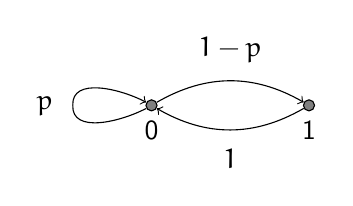
\begin{tikzpicture}
            \tikzstyle{vert}=[circle, draw, fill=black!50,
            inner sep=0pt, minimum width=4pt]
            \node[vert, label=below:0] (a) at (1,0) {};
            \node[vert, label=below:1] (b) at (3,0) {};
            \node (c) at (0,0) {};
            \path
            (a) edge [->,bend left] node[label=above:$1-p$] {} (b)
            (b) edge [->,bend left] node[label=below:$1$]   {} (a)
            (a) edge [bend left, in=90] (0,0)
            (0,0) edge [->,bend left,out=90] (a);
            \node[label=left:$p$] at (0,0) {};
        \end{tikzpicture}
    \end{center}
    Define
    \(
    h_p = \lim_{n\to\infty} \frac{H(\seqn{\alpha}{n})}{n}.
    \)
    Find \(\max\limits_p h_p\).
\end{exercise}

\subsection{Block Codes with Errors}
Let \(\seqn{\alpha}{n}\) be independent identically distributed random variables on \(\{\seqn{a}{k}\}\) with probabilities \(\seqn{p}{k}\). We consider block coding defined by the functions \(E_n\) and \(D_n\):
\[
E_n:\{\seqn{a}{k}\}^n \to \{0,1\}^{L_n},
\]
\[
D_n:\{0,1\}^{L_n} \to \{\seqn{a}{k}\}^n.
\]
\begin{definition}
    The \emph{error probability \(\varepsilon_n\)} is the probability of the following event:
    \[
    [(\seqn{\alpha}{n}) = (\seqin{a}{i}{n}) \mid D_n(E_n(\seqin{a}{i}{n}))\neq (\seqin{a}{i}{n})].
    \]
\end{definition}
\begin{theorem}[Shannon]\label{thm:blockcoding}
    In block coding allowing for errors, the following relations hold:
    \begin{enumerate}
        \item If \(h > H(\alpha) = \sum_{i=1}^{k} p_i \log \frac{1}{p_i}\), then there exist functions \((E_n, D_n)\) for \(L_n = \lceil h \cdot n \rceil\), such that \(\varepsilon_n \to 0\) as \(n \to \infty\).

        \item If \(h < H(\alpha) = \sum_{i=1}^{k} p_i \log \frac{1}{p_i}\), then for any functions \((E_n, D_n)\) for \(L_n = \lceil h \cdot n \rceil\), the error probability \(\varepsilon_n \to 1\) as \(n \to \infty\).
    \end{enumerate}
\end{theorem}
\begin{definition}
    We will say that the word \(w = \langle\seqin{a}{i}{n}\rangle\) is \emph{\(\delta\)-typical} if each letter \(a_j\) occurs in it \(t_j\) times, such that
    \[
    \begin{cases}
        t_j \le (p_j + \delta) \cdot n,\\
        t_j \ge (p_j - \delta) \cdot n.
    \end{cases}
    \]
\end{definition}
\begin{lemma}\label{lm:typicalwordprob}
    For \(\delta = n^{-0.49} = \frac{n^{0.01}}{\sqrt{n}}\), the probability of being not \(\delta\)-typical does not exceed \(\varepsilon_n\), as \(\varepsilon_n \to 0\).
\end{lemma}
\begin{proof}
    Apply Chebyshev's inequality:
    \[
    \mathrm{P}[|X - \mu| \ge \delta n] \le \frac{\sigma^2}{(\delta n)^2} =
    \frac{np_i(1-p_i)}{\delta^2 n^2} = O(n^{-0.02}). \qedhere
    \]
\end{proof}

\begin{lemma}\label{lm:typicalcount}
    For \(\delta = n^{-0.49}\) and \(h > H(\alpha)\), the number of \(\delta\)-typical words does not exceed \(2^{h \cdot n}\) (for sufficiently large \(n\)).
\end{lemma}
\begin{proof}
    First, let us consider words of a specific \emph{type}, in which letter \(i\) occurs \(n_i\) times, with \(n_1 + n_2 + \dotsb + n_k = n\). We will first estimate the number of words of the type where \(n_i = n \cdot p_i\). The number of such words is:
    \[
    \frac{n!}{n_1! n_2! \dotsm n_k!}.
    \]
    By Stirling's formula, \(n! \sim \sqrt{2\pi n}\left(\frac{n}{e}\right)^n \cdot (1 + o(1))\).
    \begin{multline}\label{eq:typicalwords}
        \log \frac{n!}{n_1! n_2! \dotsm n_k!} \approx
        \log \frac{\poly(n) \left(\frac{n}{e}\right)^n}
        {\poly(n)\left(\frac{n_1}{e}\right)^{n_1}\dotsm
            \left(\frac{n_k}{e}\right)^{n_k}} = \\
        = \log \left(\frac{n}{n_1}\right)^{n_1}\dotsm
        \left(\frac{n}{n_k}\right)^{n_k} + O(\log n)
        = \sum_{i=1}^k \underbrace{np_i}_{n_i}\cdot
        \log{\textstyle\frac{1}{p_i}} + O(\log n) < h \cdot n.
    \end{multline}
    The last inequality holds asymptotically, since we assume \(h > H(\alpha)\).
    We have only estimated this for a specific type of words. Now let us estimate for any \(\delta\)-typical word with \(n_i = n \cdot (p_i + \Delta_i)\), where \(|\Delta_i| \le \delta\). Then \eqref{eq:typicalwords} will change as follows:
    \[
    \dots =
    \sum_{i=1}^k n(p_i + \Delta_i) \cdot
    \log{\textstyle\frac{1}{p_i + \Delta_i}} + O(\log n) =
    n \cdot \sum_{i=1}^k p_i \cdot
    \log{\textstyle\frac{1}{p_i}} + O(\log n) + n \cdot O(\delta) < h \cdot n.
    \]
    (Indeed, the entropy is a continuous function, so with a small deviation, it changes by \(c \cdot \max_i \Delta_i\), where \(c\) depends on the derivative of the entropy function.)
    Thus, the total number of \(\delta\)-typical words can be estimated as the number of types multiplied by the number of \(\delta\)-typical words of one type:
    \[
    \poly(n) \cdot 2^{n \cdot H(\alpha) + n \cdot O(\delta) + O(\log n)} < 2^{h \cdot n}. \qedhere
    \]
\end{proof}

\begin{proof}[Proof of Theorem~\ref{thm:blockcoding}] \mbox{}
    \begin{enumerate}
        \item If we code only \(\delta\)-typical words, then by lemma~\ref{lm:typicalcount} it will be sufficient to have code length \(L_n\), and the probability of all non-typical words will tend to zero.

        \item Let \(\hat\varepsilon_n\) be the error probability when decoding \(\delta\)-typical words.
        We want to show that \(\hat\varepsilon_n \to 1\).
        Let us consider a specific \(\delta\)-typical word \(w=\langle\seqin{a}{i}{n}\rangle\). Let \(p_1', p_2', \dotsc, p_k'\) be the frequencies of the letters \(\seqn{a}{n}\) in the word \(w\).
        We estimate the probability of the occurrence of \(w\):
        \[
        \Pr[\langle\seqin{\alpha}{i}{n}\rangle = w] =
        p_1^{p_1' \cdot n} \cdot \dotsc \cdot p_k^{p_k' \cdot n}
        =   2^{-(\sum_i p_i' \log \frac{1}{p_i}) \cdot n}
        \le 2^{-(\sum_i p_i \log \frac{1}{p_i}) \cdot n + O(\delta_n \cdot n)}.
        \]
        In total, we can correctly code no more than \(2^{L_n}\) \(\delta\)-typical words, thus the probability of correctly decoding a \(\delta\)-typical word is
        \[
        1 - \hat\varepsilon_n \le 2^{L_n} \cdot 2^{-H(\alpha) \cdot n + O(\delta_n \cdot n)} \le
        2^{h \cdot n + 1} \cdot 2^{-H(\alpha) \cdot n + O(\delta_n \cdot n)}
        \to 0.
        \]
        Thus, \(\hat\varepsilon_n \to 1\). Together with lemma~\ref{lm:typicalwordprob}, we obtain that \(\varepsilon_n \to 1\). \qedhere
    \end{enumerate}
\end{proof}
\begin{remark}
    Using the previous theorem, one can derive an alternative proof of the inequality \(H(\alpha, \beta) \le H(\alpha) + H(\beta)\). The left side represents the asymptotic average length of the code in block coding \((\alpha, \beta)\), while the right side represents the sum of the average lengths of the codes for \(\alpha\) and \(\beta\) coded separately. Since we can consider coding \((\alpha, \beta)\) as a concatenation of codes for \(\alpha\) and \(\beta\), the inequality holds.
\end{remark}

\section{Properties of Distributions}
\subsection{Entropy Profiles}
\begin{statement}
    For any \(h \ge 0\), there exists a distribution \(\alpha\) such that \(H(\alpha) = h\).
\end{statement}
\begin{proof}
    Take some integer \(n\): \(0 \le h \le \log n\). The desired distribution is a linear combination of the distributions with probabilities \((1, 0, \dotsc, 0)\) and \((\frac{1}{n}, \frac{1}{n}, \dotsc, \frac{1}{n})\).
\end{proof}

What could the joint distribution of two random variables \(\alpha\) and \(\beta\) be? Let us consider how the \emph{entropy profile} \((H(\alpha), H(\beta), H(\alpha, \beta))\) might be structured.

\begin{statement}
    For any numbers \(h_1, h_2, h_{12} \ge 0\) that satisfy the following relations:
\[
    \left\{
    \begin{array}{lll}
        h_{12} \le h_1 + h_2 & \iff & t_0 = I(\alpha:\beta) \ge 0,\\
        h_{2} \le h_{12}     & \iff & t_1 = H(\alpha \mid \beta) \ge 0,\\
        h_{1} \le h_{12}     & \iff & t_2 = H(\beta \mid \alpha) \ge 0.
    \end{array}
    \right.
\]
    there exists a pair of random variables \((\alpha, \beta)\) with the entropy profile \((h_1, h_2, h_{12})\).

\end{statement}
\begin{proof}
    Let \(\xi_0, \xi_1, \xi_2\) be independent random variables with entropies \(t_0, t_1, t_2\) respectively. Then \(\alpha = (\xi_0, \xi_1)\) and \(\beta = (\xi_0, \xi_2)\) will be the desired variables.
    \begin{center} \mbox{}\hfill
    \parbox{.4\textwidth}{\centering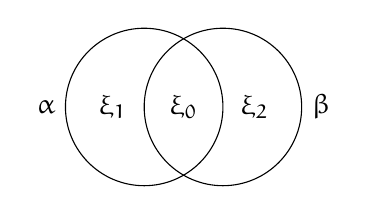
\begin{tikzpicture}
    \tikzstyle{circ}=[circle, draw, inner sep=0pt, minimum width=2cm]

    \node[circ, label=left:$\alpha$] (a) at (0,0) {};
    \node[circ, label=right:$\beta$] (b) at (1,0) {};
    \node at (-.4,0) {$\xi_1$};
    \node at (1.4,0) {$\xi_2$};
    \node at (.5,0)  {$\xi_0$};
    \end{tikzpicture}}\hfill
    	\parbox{.5\textwidth}{
            \[
            \begin{cases}
                H(\xi_0) = t_0 = h_1 + h_2 - h_{12},\\
                H(\xi_1) = t_1 = h_{12} - h_{2},\\
                H(\xi_2) = t_2 = h_{12} - h_{1}.\\
            \end{cases}
            \]\qedhere}
    \end{center}
\end{proof}

Let’s try to understand a similar question for triples of random variables. The entropy profile for the triplet \((\alpha, \beta, \gamma)\) will be defined by 7 numbers:
\[
\bigl(H(\alpha), H(\beta), H(\gamma), H(\alpha, \beta), H(\alpha, \gamma),
H(\beta, \gamma), H(\alpha, \beta, \gamma)\bigr).
\]
For the random variables \((\alpha, \beta, \gamma)\), we can write 9 independent inequalities.
\begin{equation*}
\begin{array}{lll}
H(\alpha \mid \beta, \gamma) \ge 0, & I(\alpha : \beta) \ge 0, & I(\alpha : \beta \mid \gamma) \ge 0,\\
H(\beta \mid \gamma, \alpha) \ge 0, & I(\beta : \gamma) \ge 0, & I(\beta : \gamma \mid \alpha) \ge 0,\\
H(\gamma \mid \alpha, \beta) \ge 0, & I(\gamma : \alpha) \ge 0, & I(\gamma : \alpha \mid \beta) \ge 0.
\end{array}
\end{equation*}
\begin{definition}
Define the total information of three random variables as
\[
    I(\alpha : \beta : \gamma) = I(\alpha : \beta) - I(\alpha : \beta \mid \gamma).
\]
\end{definition}

The relationships involving information quantities have a convenient geometric interpretation. Let’s draw three Euler circles and associate the areas of each resulting closed region with some information quantity.
    \begin{center}
    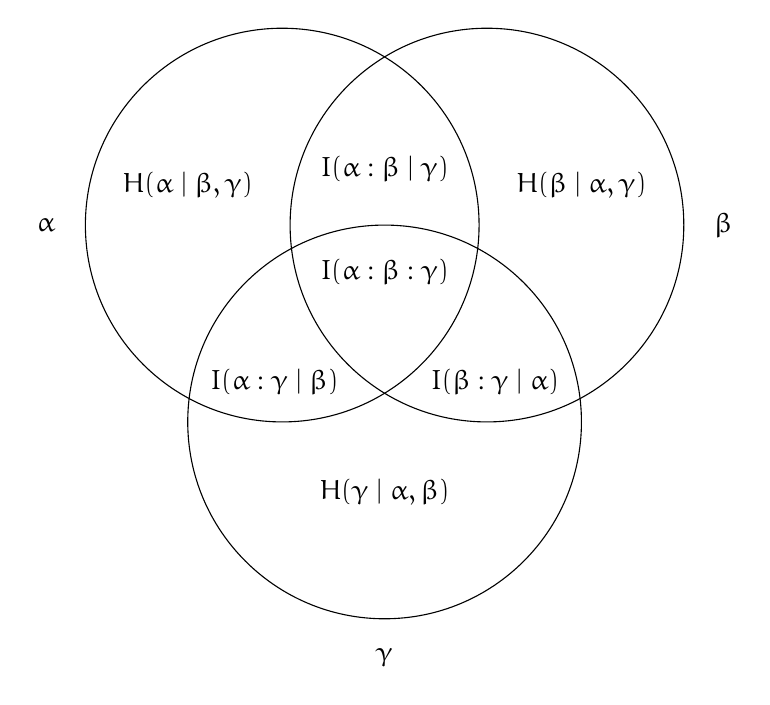
\begin{tikzpicture}
        \tikzstyle{circ}=[circle, draw, inner sep=0pt, minimum width=5cm]

        \draw(1.2,2) circle(2.5cm) node[xshift=-3cm]{$\alpha$};
        \draw(3.8,2) circle(2.5cm) node[xshift=3cm] {$\beta$};
        \draw(2.5,-0.5) circle(2.5cm) node[yshift=-3cm] {$\gamma$};

        \node at (0,2.5) {$H(\alpha \mid \beta, \gamma)$};
        \node at (5,2.5) {$H(\beta \mid \alpha, \gamma)$};
        \node at (2.5,-1.4) {$H(\gamma \mid \alpha, \beta)$};

        \node at (1.1,0) {$I(\alpha : \gamma \mid \beta)$};
        \node at (2.5,2.7) {$I(\alpha : \beta \mid \gamma)$};
        \node at (3.9,0) {$I(\beta : \gamma \mid \alpha)$};

        \node at (2.5,1.4) {$I(\alpha : \beta : \gamma)$};
    \end{tikzpicture}
    \end{center}
We can verify that this results in a correct representation. For example, the area of circle \(\alpha\) will correspond to
\[
H(\alpha) = H(\alpha \mid \beta, \gamma) + I(\alpha : \beta \mid \gamma)
+ I(\alpha : \gamma \mid \beta) + I(\alpha : \beta : \gamma),
\]
and the intersection of circles \(\alpha\) and \(\beta\) will correspond to
\[
I(\alpha : \beta) = I(\alpha : \beta \mid \gamma) + I(\alpha : \beta : \gamma).
\]
In the future, we will use this geometric interpretation to prove relationships involving information quantities.

\begin{statement}
    The total information of three random variables can be negative.
\end{statement}
\begin{proof}
    Let \(\alpha\) and \(\beta\) be independent uniformly distributed random variables over \(\{0, 1\}\). The random variable \(\gamma\) will take a value from \(\{0, 1\}\) according to the following relationship:
    \[
        \alpha \oplus \beta \oplus \gamma = 0.
    \]
    We will obtain the following picture:

    \begin{center}
    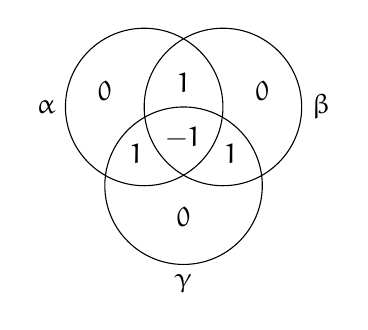
\begin{tikzpicture}
        \tikzstyle{circ}=[circle, draw, inner sep=0pt, minimum width=2cm]

        \node[circ, label=left:$\alpha$]  (a) at (1,1) {};
        \node[circ, label=right:$\beta$]  (b) at (2,1) {};
        \node[circ, label=below:$\gamma$] (c) at (1.5,0) {};
        \node at (0.5,1.2) {$0$};
        \node at (1.5,-.4) {$0$};
        \node at (2.5,1.2) {$0$};

        \node at (0.9,0.4) {$1$};
        \node at (1.5,1.3) {$1$};
        \node at (2.1,0.4) {$1$};

        \node at (1.5,0.6) {$-1$};
    \end{tikzpicture}
    \end{center}
\end{proof}
\begin{statement}
    There are no other inequalities for triples.
\end{statement}
\begin{statement}
    There are profiles that cannot be realized by any distributions, but they have measure 0.
\end{statement}
\begin{exercise}
    Prove that the following profile is realized only when \(h = \log n\) for some integer \(n\).
    \begin{center}
    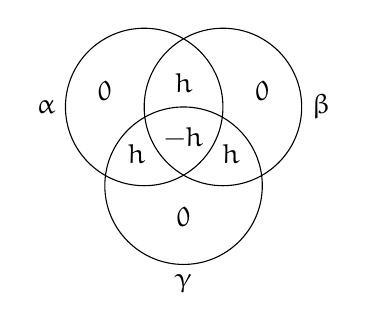
\begin{tikzpicture}
        \tikzstyle{circ}=[circle, draw, inner sep=0pt, minimum width=2cm]

        \node[circ, label=left:$\alpha$]  (a) at (1,1) {};
        \node[circ, label=right:$\beta$]  (b) at (2,1) {};
        \node[circ, label=below:$\gamma$] (c) at (1.5,0) {};
        \node at (0.5,1.2) {$0$};
        \node at (1.5,-.4) {$0$};
        \node at (2.5,1.2) {$0$};

        \node at (0.9,0.4) {$h$};
        \node at (1.5,1.3) {$h$};
        \node at (2.1,0.4) {$h$};

        \node at (1.5,0.6) {$-h$};
    \end{tikzpicture}
    \end{center}
\end{exercise}
\begin{statement}
    \(2H(\alpha, \beta, \gamma) \le H(\alpha, \beta) + H(\alpha, \gamma) + H(\beta, \gamma)\).
\end{statement}
\begin{proof}
    Note how many times each area appears in the left/right part of the inequality.
    \begin{center}
    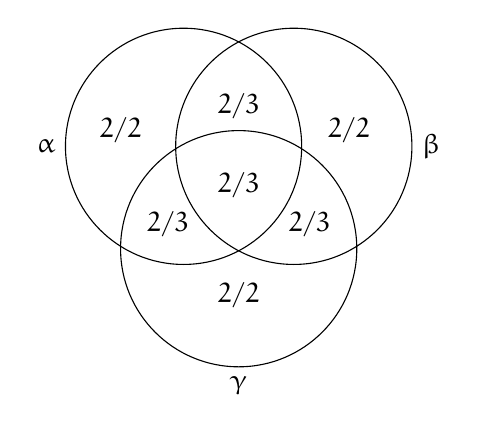
\begin{tikzpicture}
        \tikzstyle{circ}=[circle, draw, inner sep=0pt, minimum width=3cm]

        \node[circ, label=left:$\alpha$]  (a) at (1,1.3) {};
        \node[circ, label=right:$\beta$]  (b) at (2.4,1.3) {};
        \node[circ, label=below:$\gamma$] (c) at (1.7,0) {};
        \node at (0.2,1.5) {$2/2$};
        \node at (3.1,1.5) {$2/2$};
        \node at (1.7,-.6) {$2/2$};

        \node at (0.8,0.3) {$2/3$};
        \node at (2.6,0.3) {$2/3$};
        \node at (1.7,1.8) {$2/3$};

        \node at (1.7,0.8) {$2/3$};
    \end{tikzpicture}
    \end{center}
Thus, the statement simplifies to \(0 \le I(\beta : \gamma) + I(\alpha : \beta \mid \gamma) +
I(\alpha : \gamma \mid \beta)\).
\end{proof}

\begin{corollary}[Theorem~\ref{thm:volume}]
For \(A \subset \bitstr \times \bitstr \times \bitstr\)
\[2\chi(A) \le \chi_{12}(A) + \chi_{13}(A) + \chi_{23}(A).\]
\end{corollary}
\begin{proof}
    Let \((\alpha, \beta, \gamma)\) be uniformly distributed over \(A\) (i.e., the random variables are the coordinates of points in the set \(A\)).
    \[
        2\chi(A) = 2H(\alpha, \beta, \gamma) \le
        \underbrace{H(\alpha, \beta)}_{\le \chi_{12}(A)} +
        \underbrace{H(\alpha, \gamma)}_{\le \chi_{13}(A)} +
        \underbrace{H(\beta, \gamma)}_{\le \chi_{23}(A)}.
    \]
\end{proof}
We can consider a generalization of this theorem for an arbitrary number of coordinates.
\begin{theorem}[Shirer's Lemma]
    Let \(X\) be a random variable distributed over \(\bits^n\).
    For any distribution \(S\) on subsets of \([n]\), where
    \(\Pr[i \in S] \ge \mu\), it holds that \(\E[H(X_S)] \ge \mu \cdot H(X)\).
\end{theorem}
\begin{proof}
    For any set \(T = \{\seqn{i}{k}\} \subset [n]\),
    \(i_1 < i_2 < \dotsb < i_k\), we have
    \[
        H(X_T) = H(X_{i_1}) + H(X_{i_2} \mid X_{i_1}) + \dotsb + H(X_{i_k} \mid X_{i_1}, \dotsc, X_{i_{k-1}}).
    \]
    We will use the fact that \(H(X_{i_t} \mid X_{i_1}, \dotsc, X_{i_{t-1}}) \ge H(X_{i_t} \mid X_{<i_t})\), then
    \[
        H(X_T)
        \ge H(X_{i_1} \mid X_{<i_1}) + H(X_{i_2} \mid X_{<i_2}) + \dotsb + H(X_{i_k} \mid X_{<i_k}).
    \]
    Now let’s apply this fact to the distribution \(S\).
    \begin{align*}
        \E_S[H(X_S)]
        &\ge \E_S\biggl[\sum_{i \in S} H(X_i \mid X_{<i})\biggr]
         = \sum_{i \in [n]} \Pr[i \in S] \cdot H(X_i \mid X_{<i})\\
        &\ge \mu \sum_{i \in [n]} H(X_i \mid X_{<i}) = \mu \cdot H(X).\tag*{\qedhere}
    \end{align*}
\end{proof}
Shirer's Lemma has many applications.
\begin{example}[Counting Triangles in a Graph]
    Let \(G = (V, E)\) be an undirected graph with \(t\) triangles, and let \(\ell = |E|\). We will show that \(t \le \frac{(2\ell)^{3/2}}{6}\).
    \begin{proof}
        Let the triplet of random variables \((\alpha, \beta, \gamma)\) be uniformly distributed over the vertices of the triangles, and let \(X = (\alpha, \beta, \gamma)\). Then \(H(X) = H(\alpha, \beta, \gamma) = \log(6t)\), since each triangle occurs with six different permutations. Consider the distribution \(S\), uniform on subsets \(\{1, 2, 3\}\) of size 2. Then \(\Pr[i \in S] = \frac{2}{3}\). By Shirer's Lemma,
    \[
        \E_S[H(X_S)] \ge \frac{2}{3} \log(6t),
    \]
    i.e., there exists \(T \subset \{1, 2, 3\}\) for which \(H(X_T) \ge \frac{2}{3} \log(6t)\).
    On the other hand, \(X_T\) is a distribution over the edges of the graph, so \(\log(2\ell) \ge H(X_T)\). From this, we get that \(2\ell \ge (6t)^{2/3}\).
    \end{proof}
    A generalization for embedding arbitrary graphs can be found in~\cite{rao10}.
\end{example}

\begin{statement}\label{st:someentropyineq}
    For any \(\alpha\), \(\beta\), and \(\gamma\), the following inequality holds:
    \[
        H(\gamma) \le H(\gamma \mid \alpha) + H(\gamma \mid \beta) + I(\alpha : \beta).
    \]
\end{statement}
If \(H(\gamma \mid \alpha) = H(\gamma \mid \beta) = 0\)
(i.e., \(\gamma\) is uniquely determined by both \(\alpha\) and \(\beta\)),
then \(H(\gamma) \le I(\alpha : \beta)\).
\begin{proof}
    Let’s note how many times each area appears in the left/right part of the inequality.
    \begin{center}
    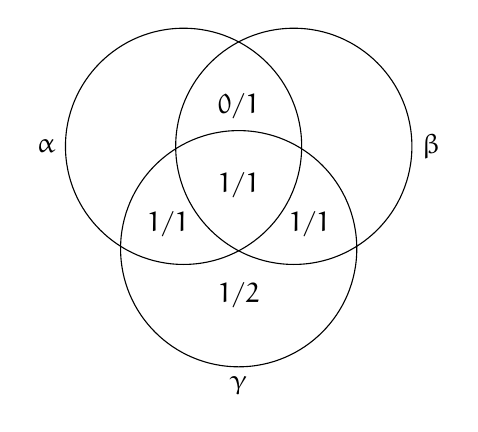
\begin{tikzpicture}
        \tikzstyle{circ}=[circle, draw, inner sep=0pt, minimum width=3cm]

        \node[circ, label=left:$\alpha$]  (a) at (1,1.3) {};
        \node[circ, label=right:$\beta$]  (b) at (2.4,1.3) {};
        \node[circ, label=below:$\gamma$] (c) at (1.7,0) {};
        \node at (1.7,-.6) {$1/2$};
        \node at (1.7,1.8) {$0/1$};
        \node at (1.7,0.8) {$1/1$};

        \node at (0.8,0.3) {$1/1$};
        \node at (2.6,0.3) {$1/1$};

    \end{tikzpicture}
    \end{center}
    Thus, the inequality simplifies to \(0 \le H(\gamma \mid \alpha, \beta) +
    I(\alpha : \beta \mid \gamma)\).
\end{proof}
\begin{exercise}
    Suppose \(\alpha \to \beta \to \gamma\) forms a Markov chain, i.e., the distribution
    \(\langle \gamma \mid \beta \rangle = \langle \gamma \mid \alpha, \beta \rangle\).
    Prove that \(I(\alpha : \gamma) \le I(\alpha : \beta)\) and \(I(\alpha : \gamma) \le I(\beta : \gamma)\).
\end{exercise}
\begin{exercise}
    Suppose \(\alpha \to \beta \to \gamma \to \delta\) forms a Markov chain.
    Prove that \(I(\alpha : \beta) \le I(\beta : \gamma)\).
\end{exercise}
\begin{exercise}\label{ex:existsdelta}
    Let \(\alpha\), \(\beta\), and \(\gamma\) have the following profile.
    \begin{center}
    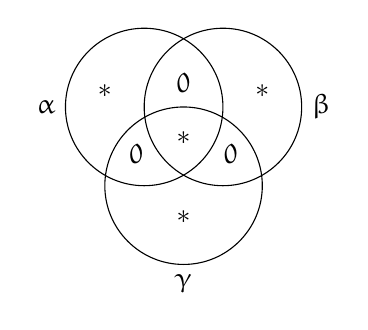
\begin{tikzpicture}
        \tikzstyle{circ}=[circle, draw, inner sep=0pt, minimum width=2cm]

        \node[circ, label=left:$\alpha$]  (a) at (1,1) {};
        \node[circ, label=right:$\beta$]  (b) at (2,1) {};
        \node[circ, label=below:$\gamma$] (c) at (1.5,0) {};
        \node at (0.5,1.2) {$*$};
        \node at (1.5,-.4) {$*$};
        \node at (2.5,1.2) {$*$};

        \node at (0.9,0.4) {$0$};
        \node at (1.5,1.3) {$0$};
        \node at (2.1,0.4) {$0$};

        \node at (1.5,0.6) {$*$};
    \end{tikzpicture}
    \end{center}
    Prove that there exists a random variable \(\delta\) such that
    \[
        \begin{cases}
            H(\delta \mid \alpha) = 0,\\
            H(\delta \mid \beta)  = 0,\\
            H(\delta \mid \gamma) = 0,\\
            H(\delta) = I(\alpha : \beta : \gamma).
        \end{cases}
    \]
    Moreover, \(I(\alpha : \beta \mid \delta) = I(\alpha : \gamma \mid \delta) = I(\beta : \gamma \mid \delta) = 0\).
\end{exercise}
\begin{exercise}
    Let’s take random variables from the previous exercise as \(x, y, a, b\): \(x = \alpha\),
    \(y = \beta\), \(a = \gamma\), \(b = \delta\). Show that for any such \((a, b, x, y)\) from the condition
    \(I(x : y \mid a) = I(x : a \mid y) = I(y : a \mid x) = 0\), it follows that
    \[
        I(a : b) \le I(a : b \mid x) + I(a : b \mid y) + I(x : y).
    \]
    [Hint: Apply the inequality from statement~\ref{st:someentropyineq}.]
\end{exercise}
\begin{exercise}
    Let’s take random variables from exercise~\ref{ex:existsdelta} as \(x, y, a, b\): \(x = \alpha\),
    \(y = \beta\), \(a = \gamma\), \(b = \delta\). Show that there exist such \((a, b, x, y)\) for which
    \[
        I(a : b) \not\le I(a : b \mid x) + I(a : b \mid y) + I(x : y).
    \]
    (That is, the condition in the previous exercise was necessary.)
\end{exercise}
\begin{statement}[Inequality for 5 Random Variables]
    \[
        I(a : b) \le I(a : b \mid x) + I(a : b \mid y) + I(x : y)
        + I(a : b \mid z) + I(a : z \mid b) + I(b : z \mid a).
    \]
\end{statement}
\begin{corollary}[Zhang, Yeung, 1998]
    An inequality for 4 random variables that cannot be expressed through the basic inequalities.
    \[
        I(a : b) \le 2I(a : b \mid x) + I(a : b \mid y) + I(x : y)
        + I(a : x \mid b) + I(b : x \mid a).
    \]
\end{corollary}
\begin{statement}
    For 4 random variables, there are infinitely many inequalities that are independent of each other.
\end{statement}

\subsection{Inequalities for Triplets}
We will prove the following statement under various assumptions:
\[
    H(a \mid x) + H(a \mid y) \le H(a).
\]

\begin{statement}
    If \(a, x, y\) are such that
\[
    \begin{cases}
        H(a \mid x, y) = 0,\\
        I(x : y \mid a) = 0.
    \end{cases}
\]
then \(H(a \mid x) + H(a \mid y) \le H(a)\).
\end{statement}
\begin{proof}
    We need to prove the non-negativity of \(h\).
    \begin{center}
    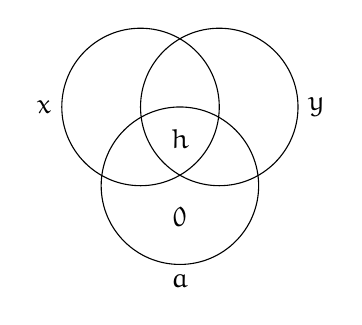
\begin{tikzpicture}
        \tikzstyle{circ}=[circle, draw, inner sep=0pt, minimum width=2cm]

        \node[circ, label=left:$x$]  (x) at (1,1) {};
        \node[circ, label=right:$y$] (y) at (2,1) {};
        \node[circ, label=below:$a$] (a) at (1.5,0) {};
        \node at (1.5,-.4) {$0$};

        \node at (1.5,0.6) {$h$};
    \end{tikzpicture}
    \end{center}
Since \(I(x : y \mid a) = 0\), it follows that \(h = I(x : y) \ge 0\).
\end{proof}
\begin{statement}\label{st:entropy:triple-rect}
    If \(a, x, y\) are such that \(H(a \mid x, y) = 0\) and
\[
    \begin{cases}
        A_i \sim X_j\\
        A_i \sim Y_k
    \end{cases} \implies A_i \sim (X_j, Y_k),
\]
then \(H(a \mid x) + H(a \mid y) \le H(a)\). (The notation \(A_i \sim X_j\) means \(\Pr[a = A_i \land x = X_j] > 0\).)
\end{statement}
\begin{remark}
    The condition \(H(a \mid x, y) = 0\) can be interpreted as \(a = f(x, y)\).
\end{remark}
% todo: ask Shenya how to explain this more simply
\begin{proof}
    We will construct a new distribution \((a', x', y')\):
    \begin{itemize}
        \item \(a'\) has the same distribution as \(a\),
        \item the conditional distribution of \(x'\) given \(a'\) coincides
            with the conditional distribution of \(x\) given \(a\),
        \item the conditional distribution of \(y'\) given \(a'\) coincides
            with the conditional distribution of \(y\) given \(a\),
        \item \(x'\) and \(y'\) are independent.
    \end{itemize}
    \[
    \Pr[a' = A_i, x' = X_j, y' = Y_k] =
    \Pr[a' = A_i] \cdot \Pr[x' = X_j \mid a' = A_i] \cdot \Pr[y' = Y_k \mid a' = A_i].
    \]
    Thus,
    \[
        H(a', x', y') = H(a') + H(x' \mid a') + H(y' \mid a') - \underbrace{I(x' : y' \mid a')}_{0}.
    \]
    On the other hand,
    \[
        H(a', x', y') \le H(x') + H(y') + H(a' \mid x', y').
    \]
    Furthermore, we can erase the indicators almost everywhere.
    \[
        H(x) + H(y) + H(a' \mid x', y') \ge H(a', x', y') = H(a) + H(x \mid a) + H(y \mid a).
    \]
    We will show that \(H(a' \mid x', y') = 0\), i.e., \(a' = f(x', y')\). Indeed:
    if the triplet \((A_i, X_j, Y_k)\) in the new distribution appears with positive
    probability, then it also appeared in the original distribution with positive
    probability, hence \(a' = f(x', y')\).
    We get: \(H(a) + H(x \mid a) + H(y \mid a) \le H(x) + H(y)\). Adding \(H(a)\) to both sides of the inequality:
    \[
       H(x, a) + H(y, a) \le H(x) + H(y) + H(a) \implies H(a \mid x) + H(a \mid y) \le H(a). \qedhere
    \]
\end{proof}
\begin{problem}[Vereshchagin~\cite{KRV18}]
    Consider a bipartite graph with vertices \((L, R)\) with colored edges.
    All edges incident to a single vertex are of different colors, the degree in the left part is at least \(n\),
    and in the right part is at least \(m\). Suppose it is known that for a pair of vertices \((x \in L, y \in R)\)
    there is at most one common color. Prove that the number of colors is at least \(n \cdot m\).

    Note that monochrome edges form matchings. For each color \(c\), connect all
    vertices on the left that are matched with \(c\) to those on the right that are matched with \(c\). This forms a biclique of
    edges of color \(c\).

    Consider the distribution on triplets \((a, x, y)\) (color, vertex from the left part, vertex from the right
    part): we choose the color proportionally to the size (number of edges) of the corresponding biclique and
    select a random edge of that color. It can be checked that the following relation holds:
\[
    \begin{cases}
        A_i \sim X_j,\\
        A_i \sim Y_k,
    \end{cases} \implies A_i \sim (X_j, Y_k).
\]
Now we apply: \(\underbrace{H(a \mid x)}_{\ge \log n} +
                  \underbrace{H(a \mid y)}_{\ge \log m} \le H(a) \le \log (\text{\# colors})\).
\end{problem}
\subsection{Conditional Inequality for a Quadruple}
\begin{statement}
    If for random variables \(a, b, x, y\) the following holds
    \[
        \begin{cases}
            I(x:y \mid a) = 0,\\
            H(a \mid x, y) = 0,
        \end{cases}
    \]
    then \(I(a:b) \le I(a:b \mid x) + I(a:b \mid y) + I(x:y)\).
\end{statement}
\begin{proof}
    We will construct a new distribution \((a', b', x', y')\):
    first, we choose a value \((a', b') \sim (a, b)\).
    For a fixed value of \((a', b')\), we independently choose \(x'\) and \(y'\) such that the conditional probability distributions with respect to \(a'\) are the same as those of \(x\) and \(y\) with respect to \(a\).
    \begin{multline*}
    H(a', b', x', y') = H(a', b') + H(x \mid a', b') + H(y \mid a', b') - \underbrace{I(x':y' \mid a', b')}_{0} =\\
    = H(a, b) + H(x \mid a, b) + H(y \mid a, b).
    \end{multline*}
    On the other hand,
    \begin{multline*}
    H(a', b', x', y') \le H(b') + H(x' \mid b') + H(y' \mid b') + H(a' \mid x', y') =\\
    = H(b) + H(x \mid b) + H(y \mid b) + H(a' \mid x', y').
    \end{multline*}
    We will show that \(H(a' \mid x', y') = 0\). This was satisfied in the original distribution by assumption.
    Let \([a' = A_i, x' = X_j, y' = Y_k]\) in the new distribution occur with positive probability. Therefore, it also occurs in the original distribution with positive probability (given a fixed \(a'\), \(x'\) and \(y'\) are independent), which preserves the corresponding functional dependence of \(a'\) on \((x', y')\).

    As a result, we obtain
    \[
        H(a, b) + H(x \mid a, b) + H(y \mid a, b) \le H(b) + H(x \mid b) + H(y \mid b).
    \]
    We can rewrite this inequality using unconditional entropies:
    \[
        H(a, b) + H(x, a, b) - H(a, b) + H(y, a, b) - H(a, b) \le H(b) + H(x, b) - H(b) + H(y, b) - H(b).
    \]
    Simplifying gives us:
    \begin{equation}\label{eq:condineq1}
        H(x, a, b) + H(y, a, b) + H(b) \le H(x, b) + H(y, b) + H(a, b).
    \end{equation}
    Now we will do the same for \(I(a:b) \le I(a:b \mid x) + I(a:b \mid y) + I(x:y)\).
    \begin{equation*}
        \begin{array}{ll}
        H(a) + H(b) - H(a, b) \le
        & H(a, x) + H(b, x) - H(a, b, x) - H(x) + \mbox{} \\
        & H(a, y) + H(b, y) - H(a, b, y) - H(y) + \mbox{} \\
        & H(x) + H(y) - H(x, y).
        \end{array}
    \end{equation*}
    Simplifying yields:
    \begin{equation}\label{eq:condineq2}
        \begin{array}{ll}
        H(a, b, x) + H(a, b, y) + H(b) + H(x, y) \le
        & H(b, x) + H(b, y) + H(a, b) + \mbox{} \\
        & H(a, x) + H(a, y) - H(a).
        \end{array}
    \end{equation}

    Note that we only need to prove \(H(x, y) \le H(a) + H(x \mid a) + H(y \mid a)\).
    Adding this inequality to \eqref{eq:condineq1} will yield \eqref{eq:condineq2}.
    Let’s note how many times each area contributes to the left/right side of the inequality.
    \begin{center}
    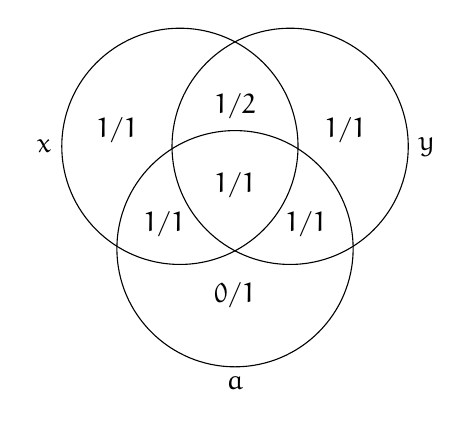
\begin{tikzpicture}
        \tikzstyle{circ}=[circle, draw, inner sep=0pt, minimum width=3cm]

        \node[circ, label=left:$x$]  (a) at (1,1.3) {};
        \node[circ, label=right:$y$] (b) at (2.4,1.3) {};
        \node[circ, label=below:$a$] (c) at (1.7,0) {};
        \node at (0.2,1.5) {$1/1$};
        \node at (3.1,1.5) {$1/1$};
        \node at (1.7,-.6) {$0/1$};

        \node at (0.8,0.3) {$1/1$};
        \node at (2.6,0.3) {$1/1$};
        \node at (1.7,1.8) {$1/2$};

        \node at (1.7,0.8) {$1/1$};
    \end{tikzpicture}
    \end{center}
    That is, it is equivalent to \(H(a \mid x, y) + I(x:y \mid a) \ge 0\).
\end{proof}
Questions to think about: Come up with an interpretation for this inequality. Zhang and Yeung proved this same inequality in 1997 under the assumption \(I(x:y) = I(x:y \mid a) = 0\). Is there a combinatorial interpretation of this statement?

\begin{exercise}
A rectangular table is divided into (combinatorial) rectangles such that each row intersects at least \(n\) rectangles and each column intersects at least \(m\) rectangles. Prove that the total number of rectangles is at least \(nm\).
\end{exercise}


\newpage
%%%%%%%%%%%%%%%%%%%%%%%%%%%%%%%%%%%%%%%%%%%%%%%%
\begin{thebibliography}{9}
    \bibitem{veresch12} Н.К. Верещагин, Е.В. Щепин. \emph{Информация, кодирование, предсказание}, МЦНМО, 2012.

    \bibitem{veresch17} Н.К. Верещагин. \emph{Коммуникационная сложность}, Computer Science клуб, 2017.
        \url{http://compsciclub.ru/courses/communicationcomplexity/2017-spring/}

    \bibitem{romaschcsclub} А.Е. Ромащенко. \emph{Введение в теорию информации,} Computer Science клуб, 2015.
        \url{http://compsciclub.ru/courses/informationtheory/2015-spring/}

    \bibitem{romaschnotes} А.Е. Ромащенко. \emph{Краткий конспект лекций курса ``Введение в теорию информации'',} 2014.
        \url{http://www.mccme.ru/~anromash/courses/lecture-notes-it-2014.pdf}

    \bibitem{kolmbook12} В.А. Успенский, Н.К. Верещагин, А.Шень. \emph{Введение в колмогоровскую сложность}. МЦНМО, 2012.

    \bibitem{shen08} А. Шень. \emph{Алгоритмическая теория информации,} Computer Science клуб, 2008.
        \url{http://compsciclub.ru/courses/algo-information-theory/2008-autumn/}

    \bibitem{BB94} M. L. Bonet, S. R. Buss. \emph{Size-depth tradeoffs for Boolean formulae.} Information Processing Letters, 49(3), 151-155, 1994.

    \bibitem{DMWW12} D. Gavinsky, O. Meir, O. Weinstein, A. Wigderson. \emph{Toward better formula lower bounds:
    an information complexity approach to the KRW composition conjecture.} STOC 2014.

    \bibitem{KRV18} T.Kaced, A.E. Romashchenko, N.K.Vereshchagin, \emph{A Conditional Information Inequality and Its Combinatorial Applications}.
    {{IEEE} Trans. Information Theory}, 2018.

    \bibitem{NK97} E. Nisan, N. Kushilevitz. \emph{Communication complexity}, 1997.

    \bibitem{rao10} A. Rao. \emph{Notes for CSE533: Information Theory in Computer Science}, 2010. \\ \url{https://homes.cs.washington.edu/~anuprao/pubs/CSE533Autumn2010/}

\end{thebibliography}


\end{document}

% vim: set tw=120:
